%!TEX root = ../scivis_lbaakman_bvanloon.tex

\todo[inline]{Introduce section}

\subsection{Different Color Maps}
	\todo[inline]{Show image of the different colormaps, discuss}

	\begin{figure}
	\centering
	\begin{subfigure}{0.44\textwidth}
		\centering
		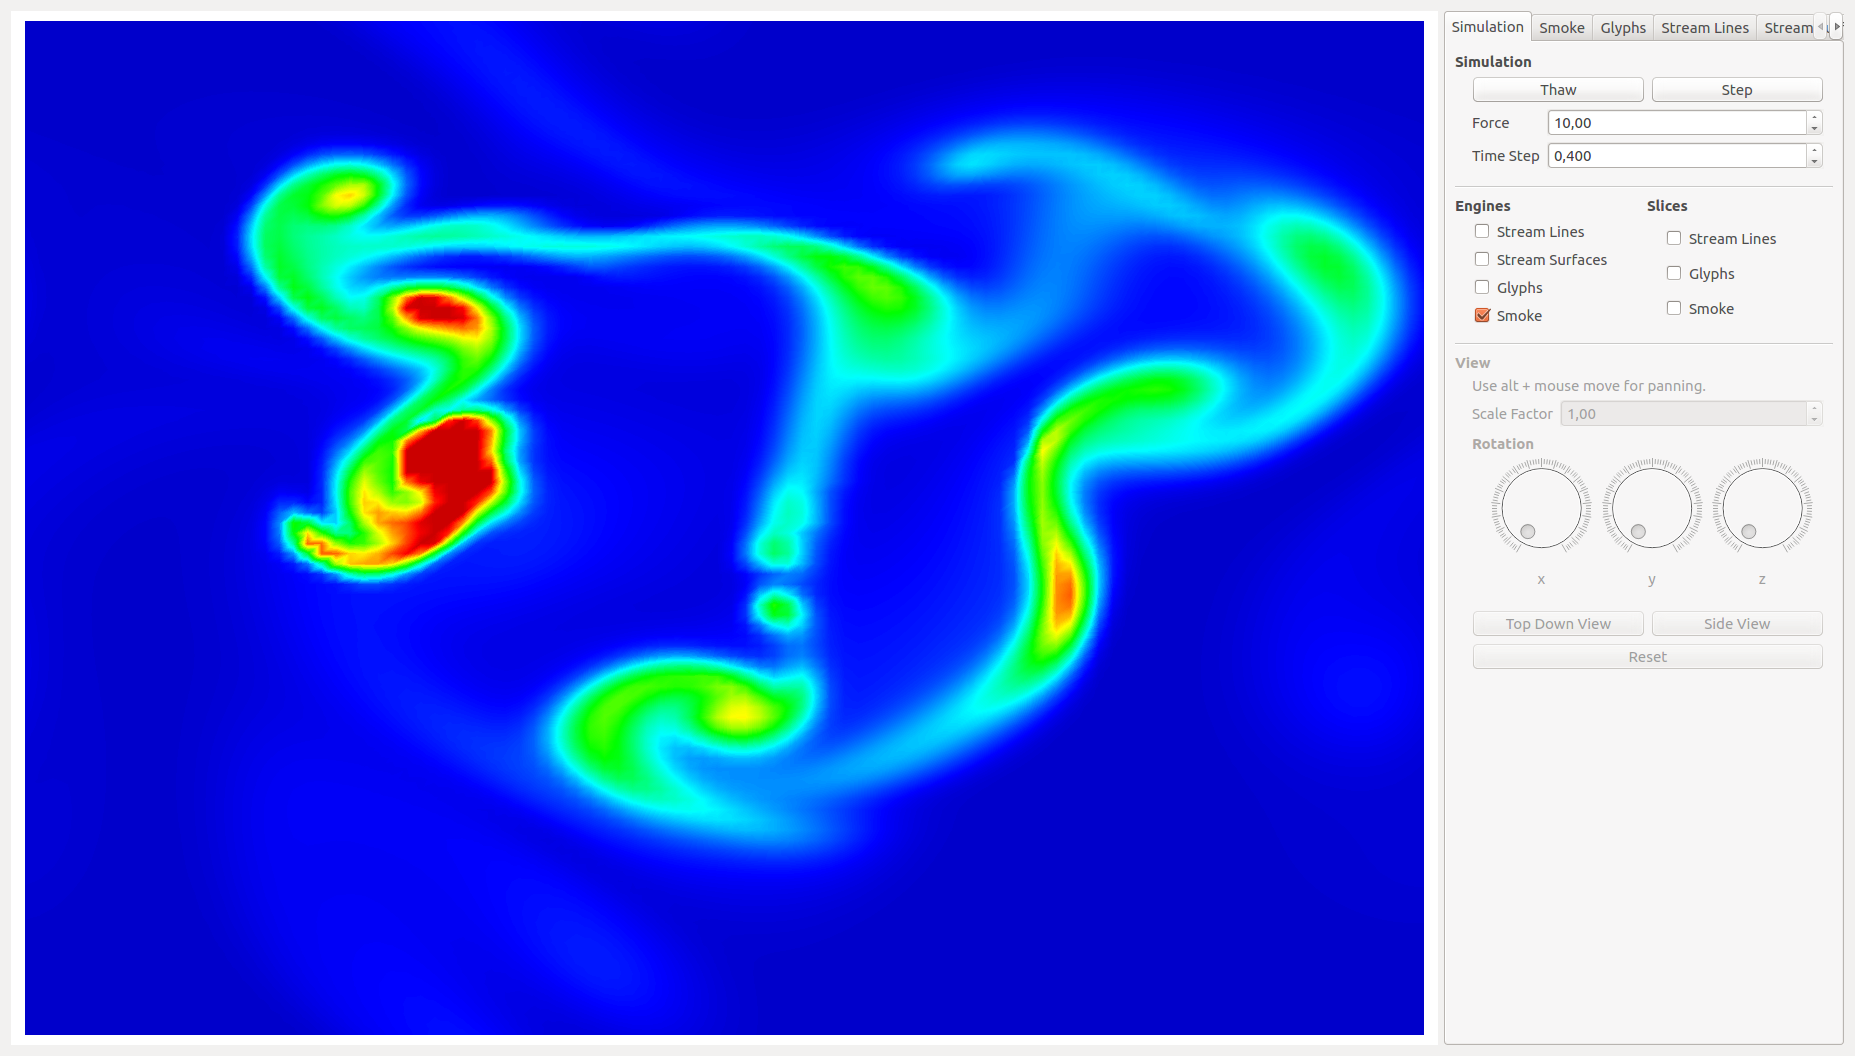
\includegraphics[width=\textwidth, trim={35px 30px 430px 30px}, clip]{colormapping/img/rainbow}
		\caption{Rainbow colormap, using $\VarDX = 0.8$.}
		\label{fig:colormapping:intro:differntColorMaps:rainbow}
	\end{subfigure}
	\begin{subfigure}{0.44\textwidth}
		\centering
		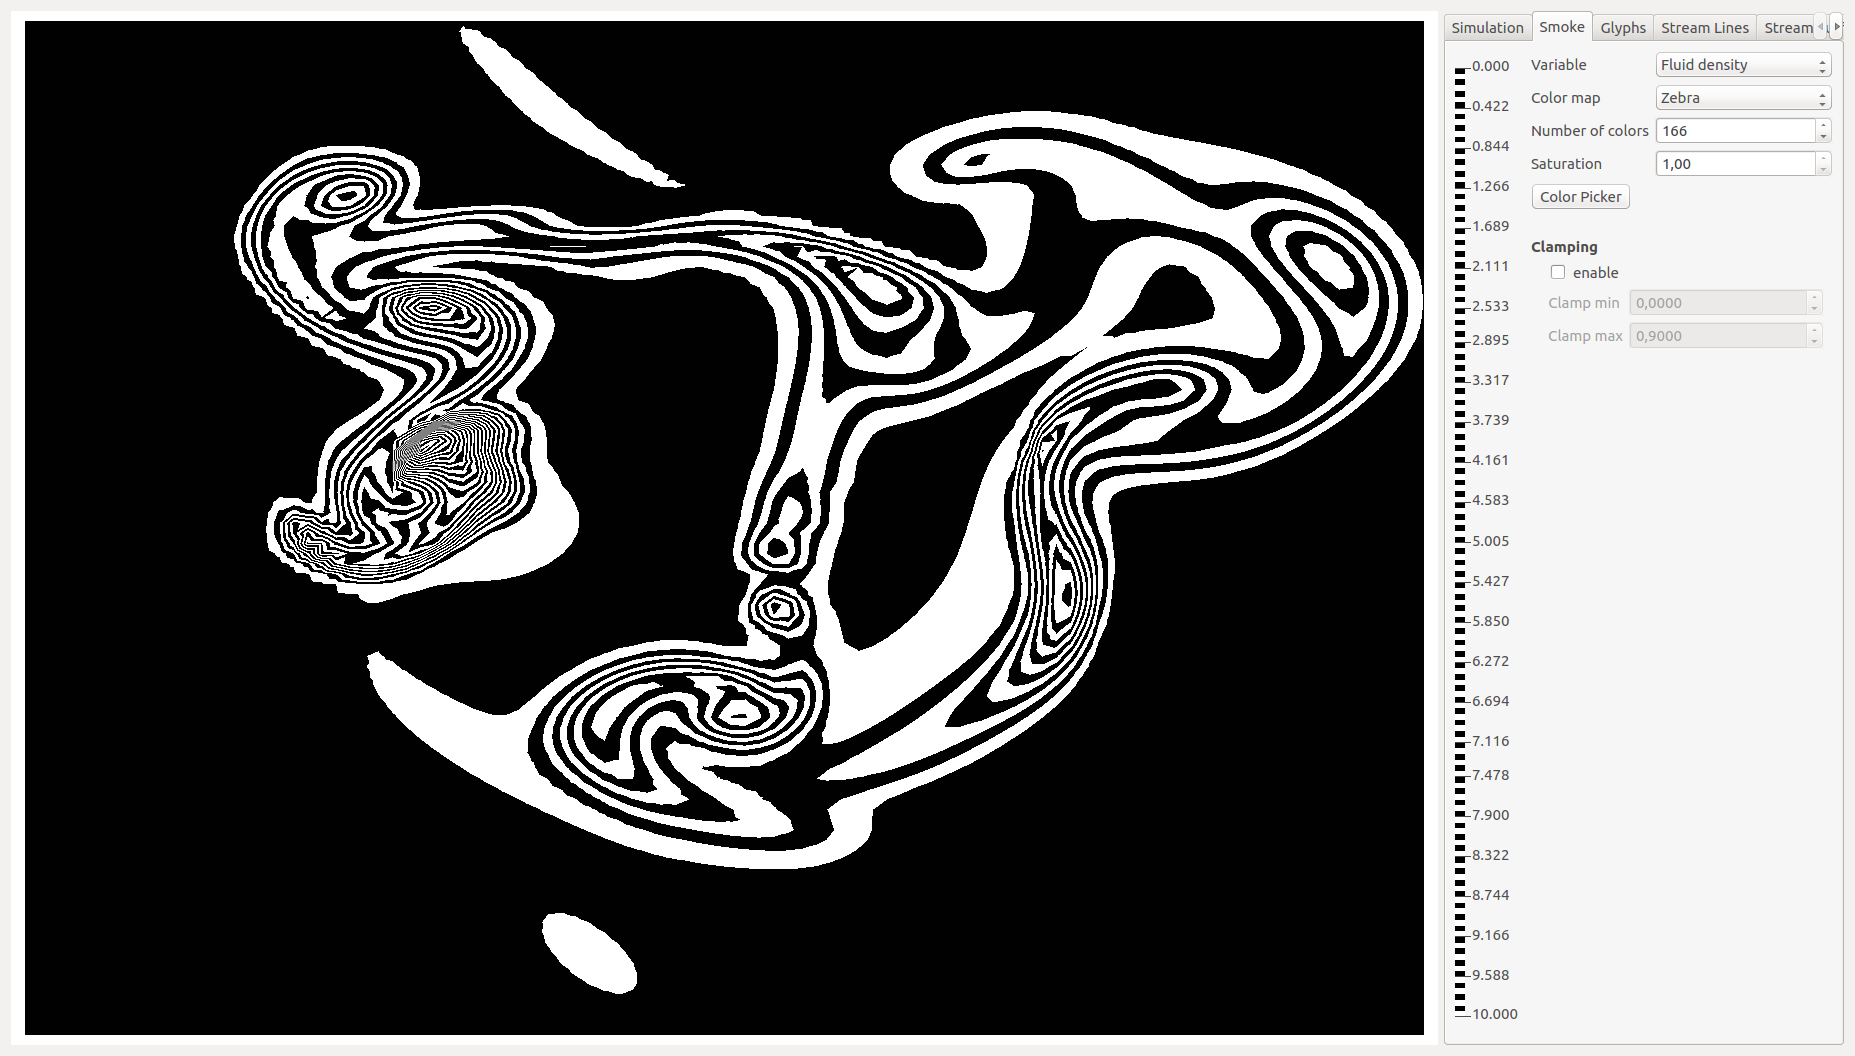
\includegraphics[width=\textwidth, trim={35px 30px 430px 30px}, clip]{colormapping/img/zebra_166}
		\caption{Zebra colormap showing the first derivative.}
		\label{fig:colormapping:intro:differntColorMaps:zebra}
	\end{subfigure}	
	\begin{subfigure}{0.44\textwidth}
		\centering
		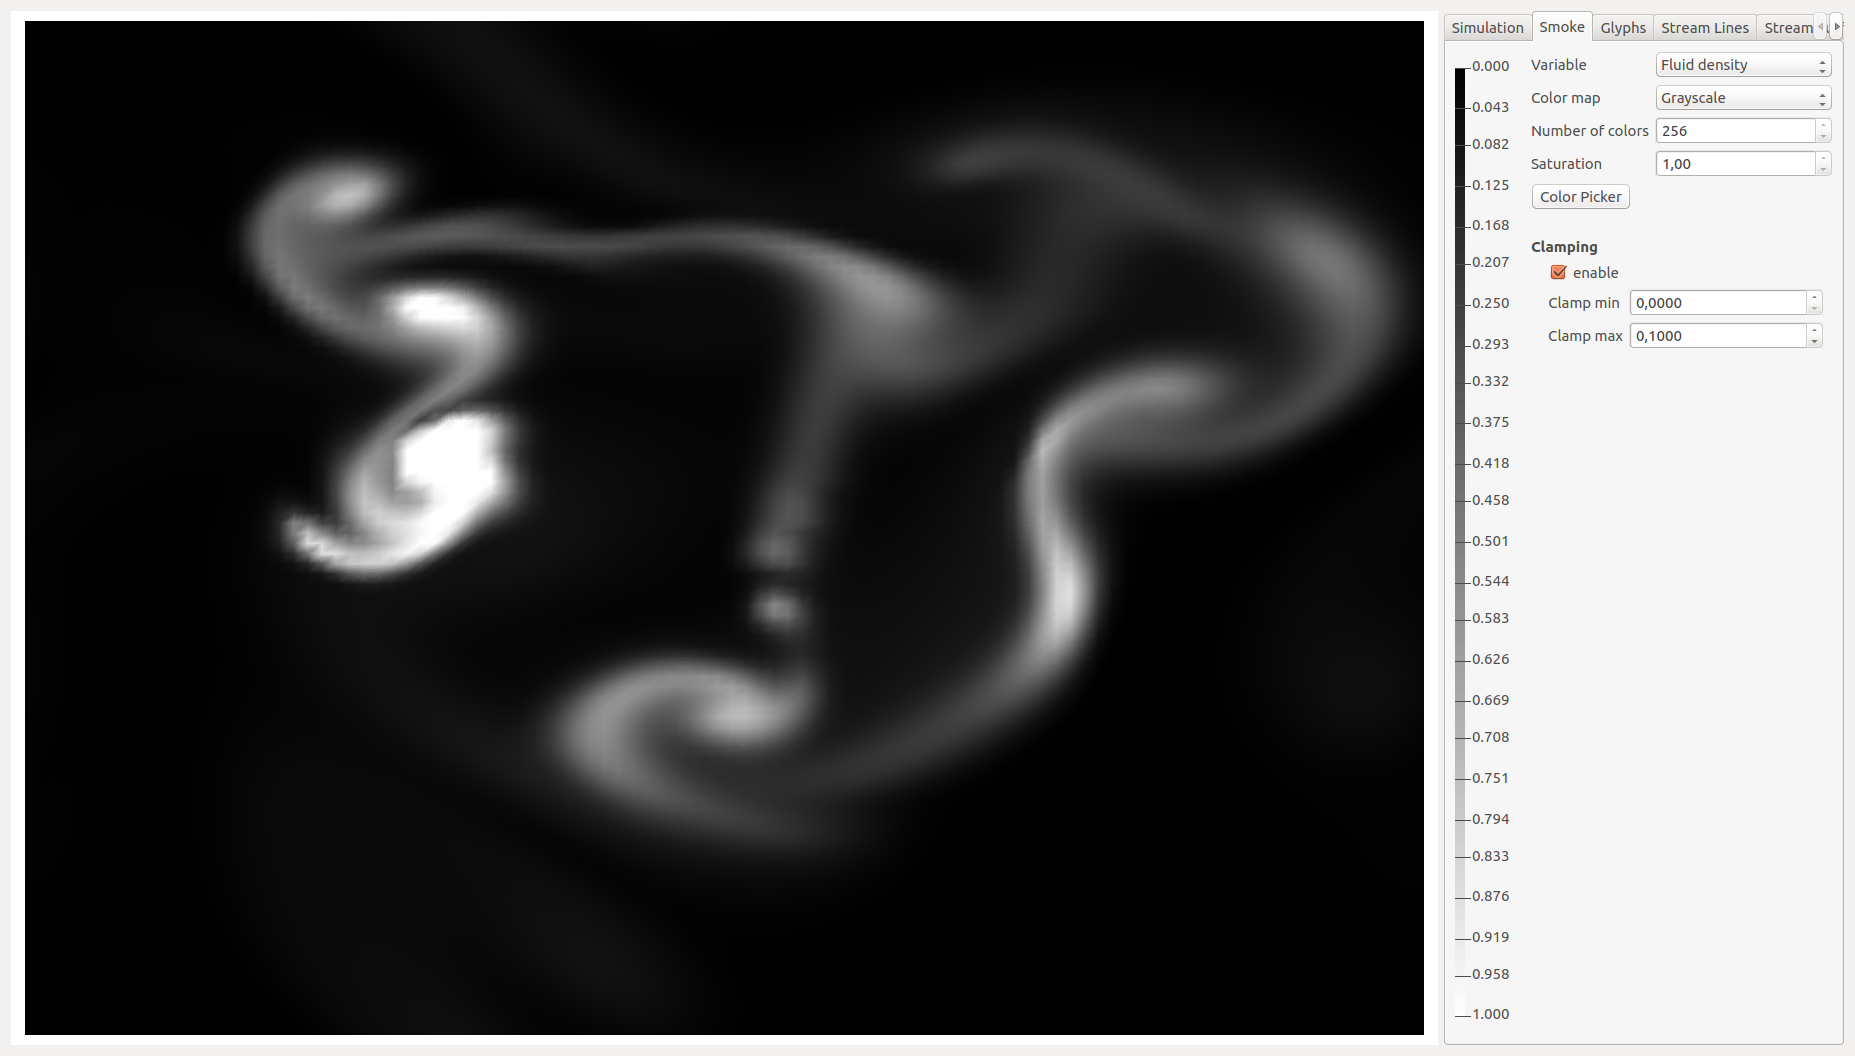
\includegraphics[width=\textwidth, trim={35px 30px 430px 30px}, clip]{colormapping/img/grayscale}
		\caption{Gray-scale colormap.}
		\label{fig:colormapping:intro:differntColorMaps:grayscale}
	\end{subfigure}	
	\begin{subfigure}{0.44\textwidth}
		\centering
		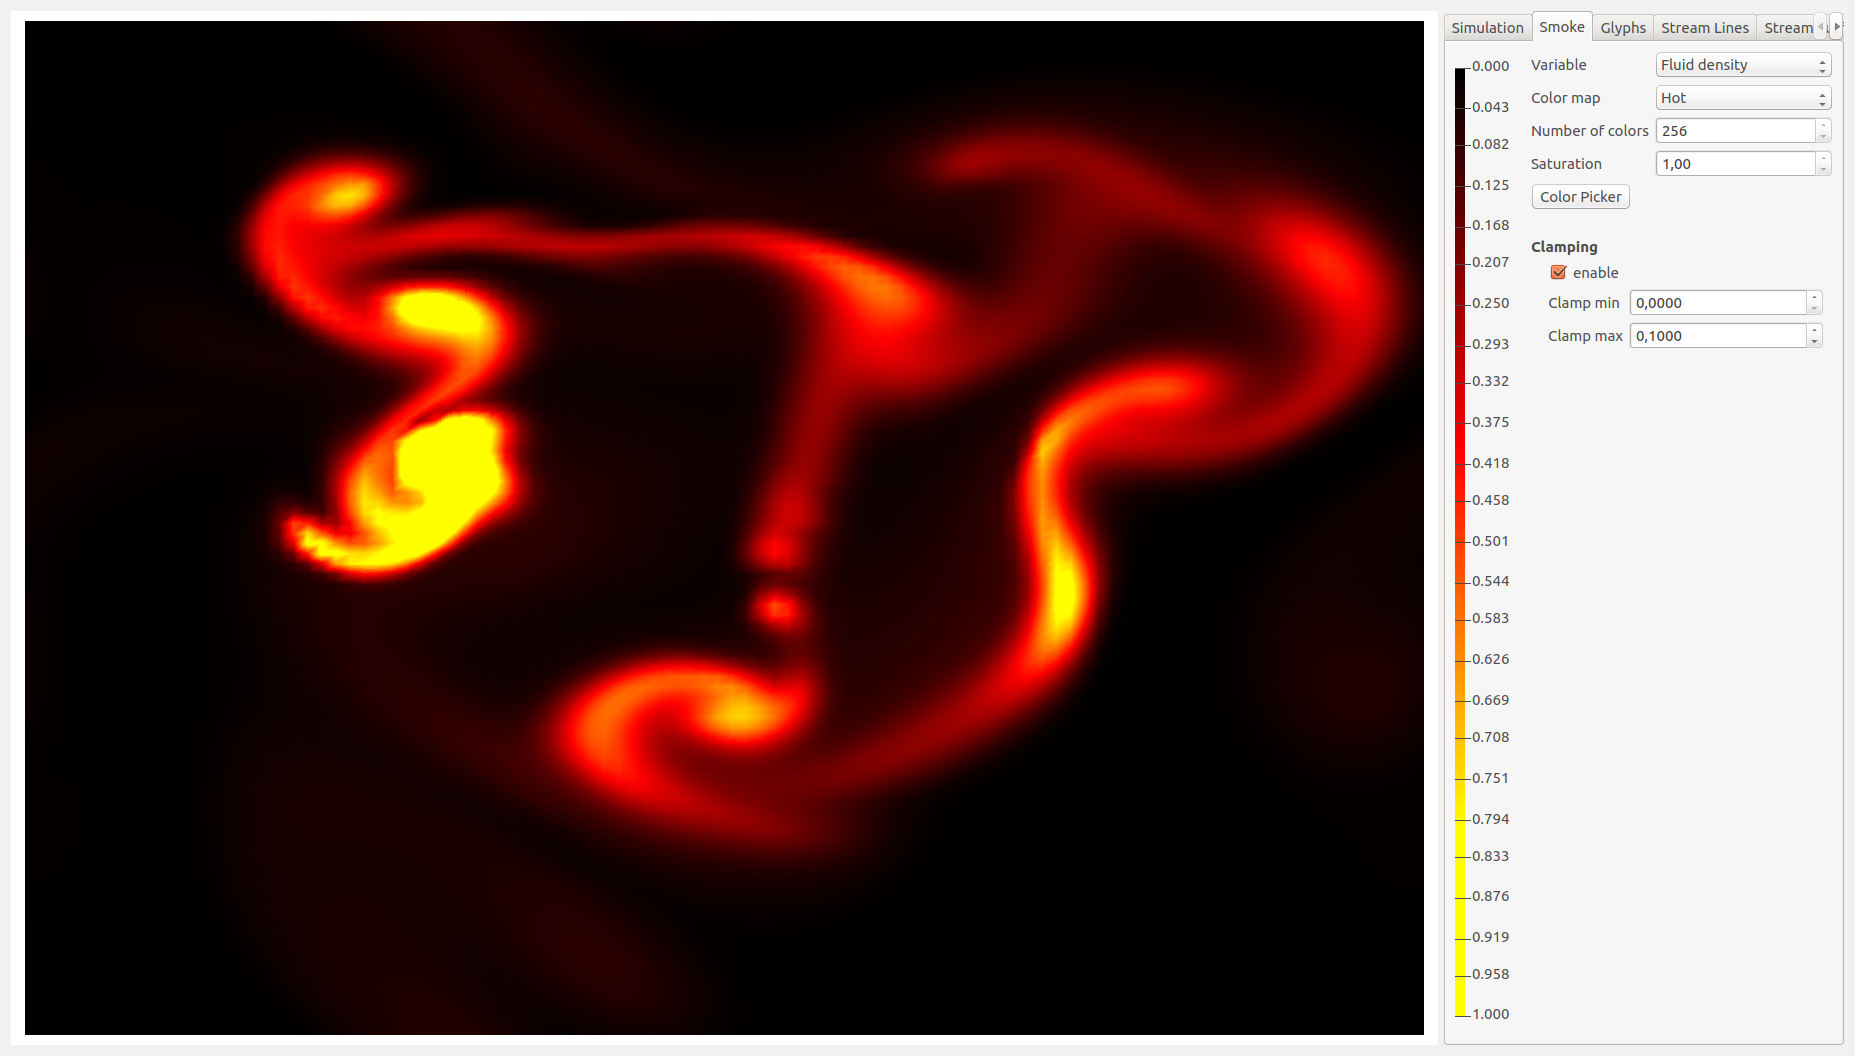
\includegraphics[width=\textwidth, trim={35px 30px 430px 30px}, clip]{colormapping/img/heat}
		\caption{Heat colormap.}
		\label{fig:colormapping:intro:differntColorMaps:heat}
	\end{subfigure}
	\begin{subfigure}{0.44\textwidth}
		\centering
		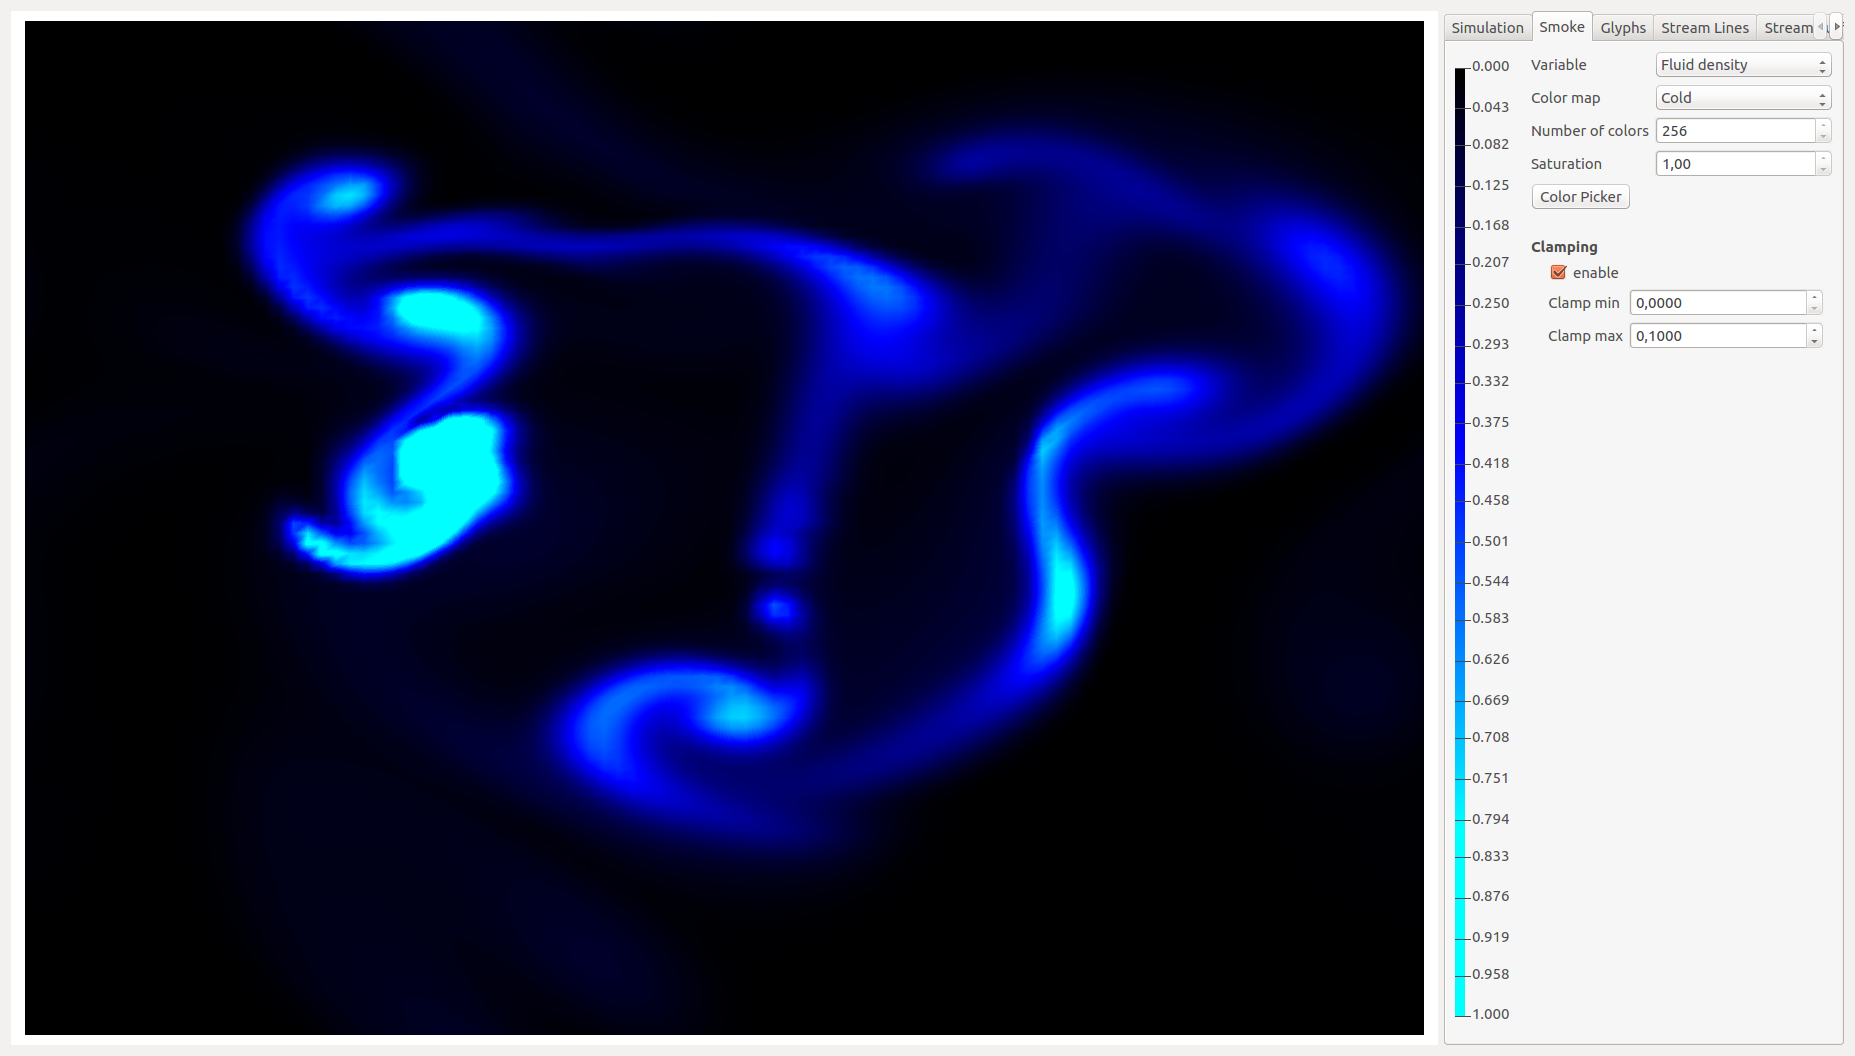
\includegraphics[width=\textwidth, trim={35px 30px 430px 30px}, clip]{colormapping/img/cold}
		\caption{Cold colormap.}
		\label{fig:colormapping:intro:differntColorMaps:cold}
	\end{subfigure}
		\begin{subfigure}{0.44\textwidth}
		\centering
		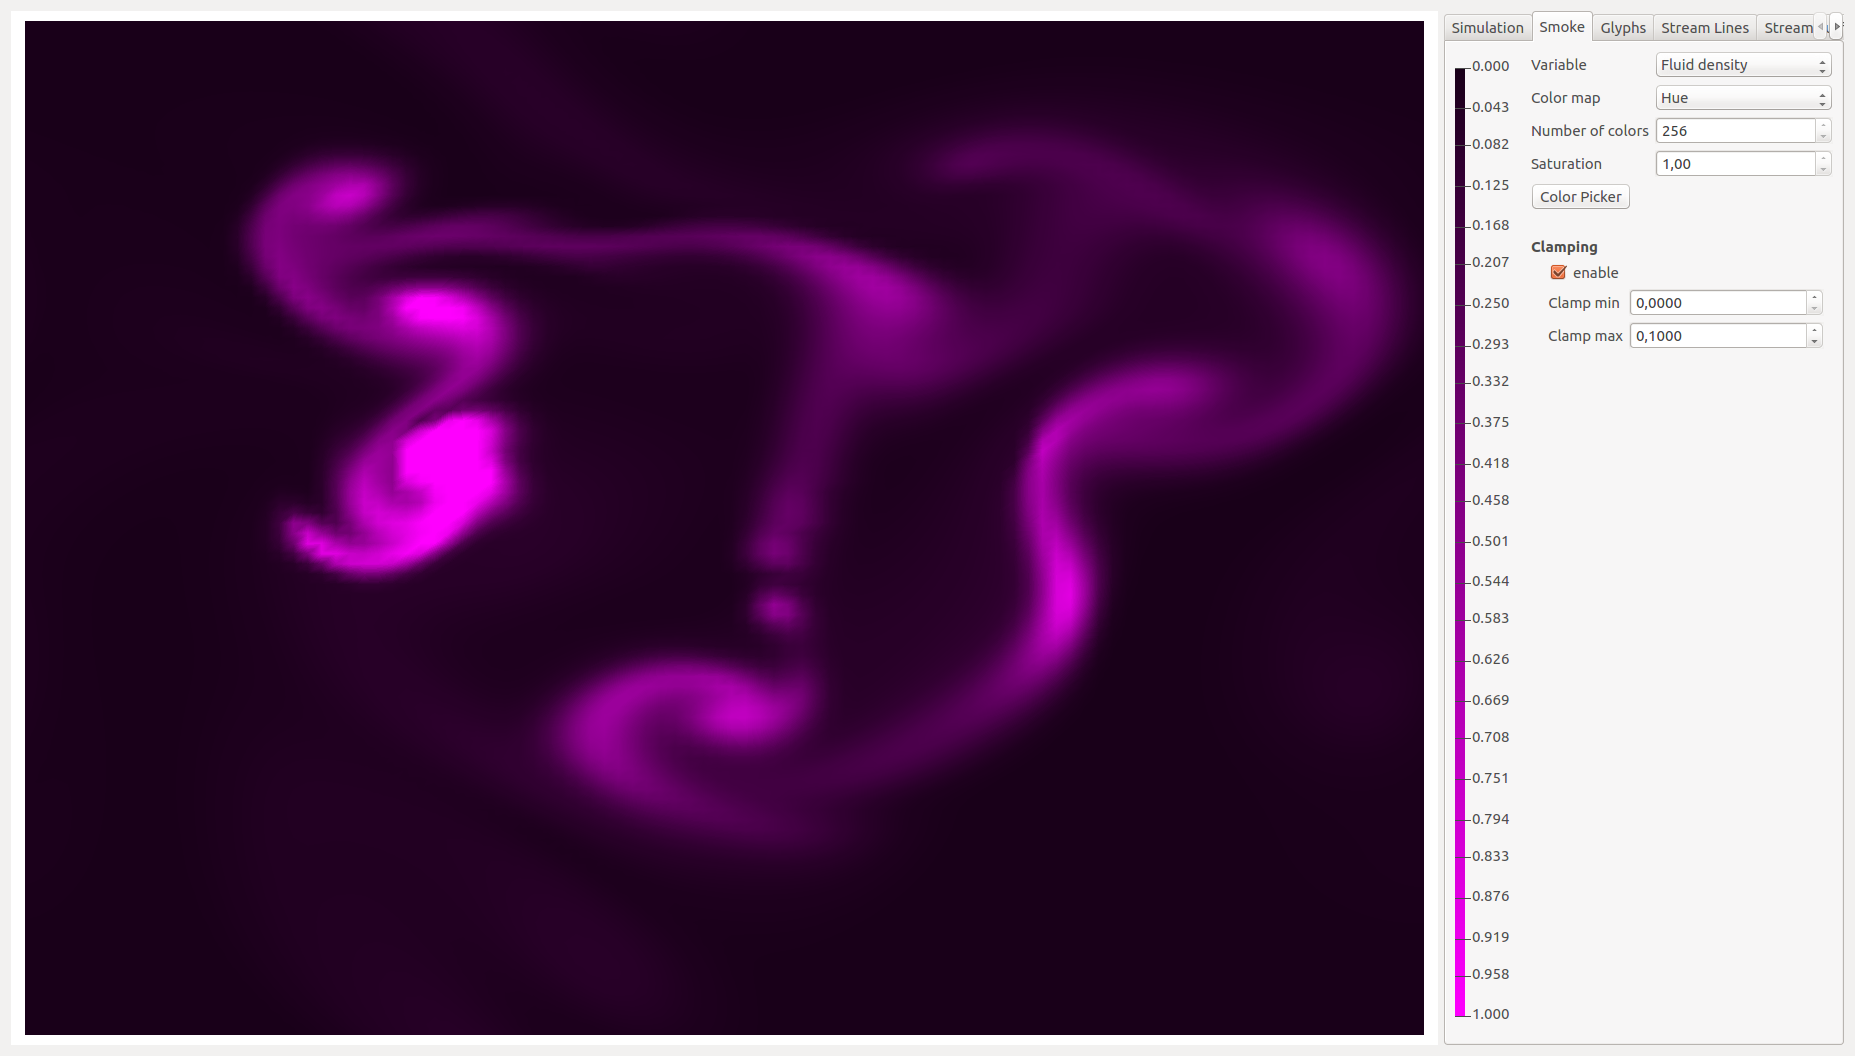
\includegraphics[width=\textwidth, trim={35px 30px 430px 30px}, clip]{colormapping/img/hue}
		\caption{Hue colormap using pink hue .}
		\label{fig:colormapping:intro:differntColorMaps:hue}
	\end{subfigure}
	\begin{subfigure}{0.44\textwidth}
		\centering
		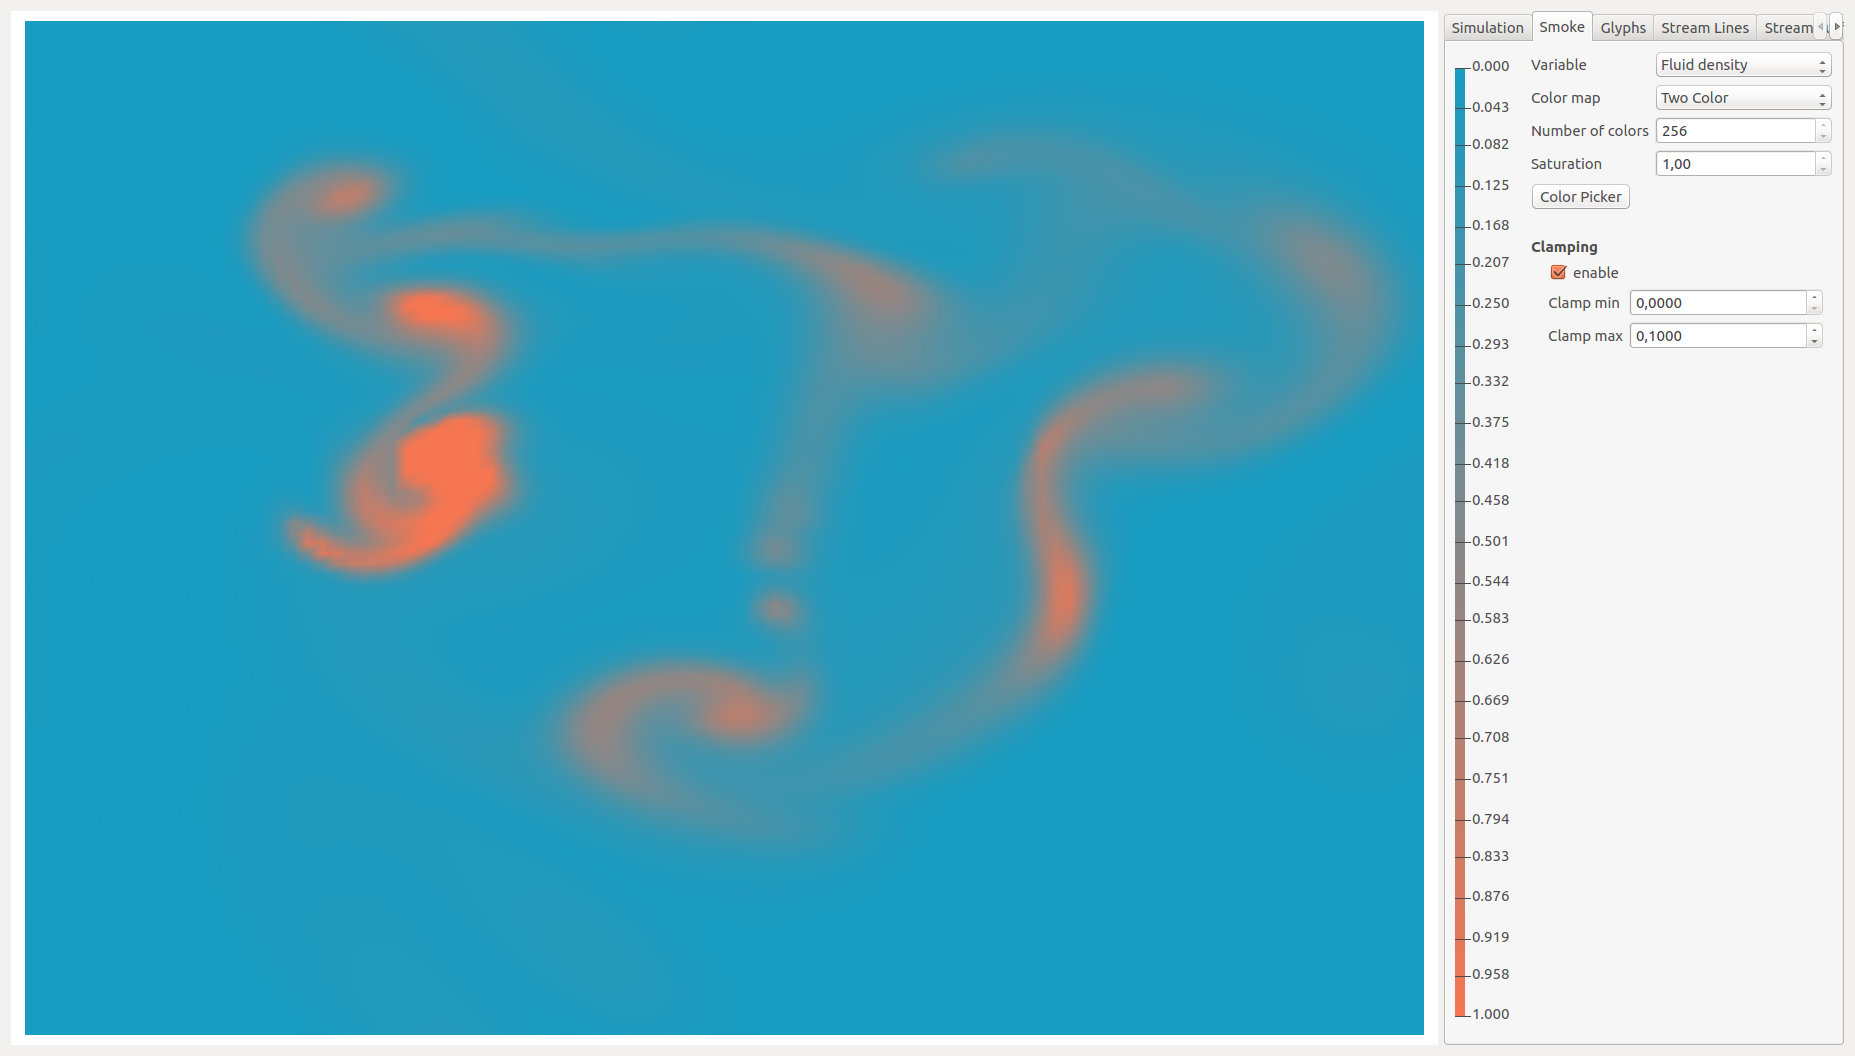
\includegraphics[width=\textwidth, trim={35px 30px 430px 30px}, clip]{colormapping/img/twocolors}
		\caption{Two-color colormap.}
		\label{fig:colormapping:intro:differntColorMaps:twocolor}
	\end{subfigure}	\begin{subfigure}{0.44\textwidth}
		\centering
		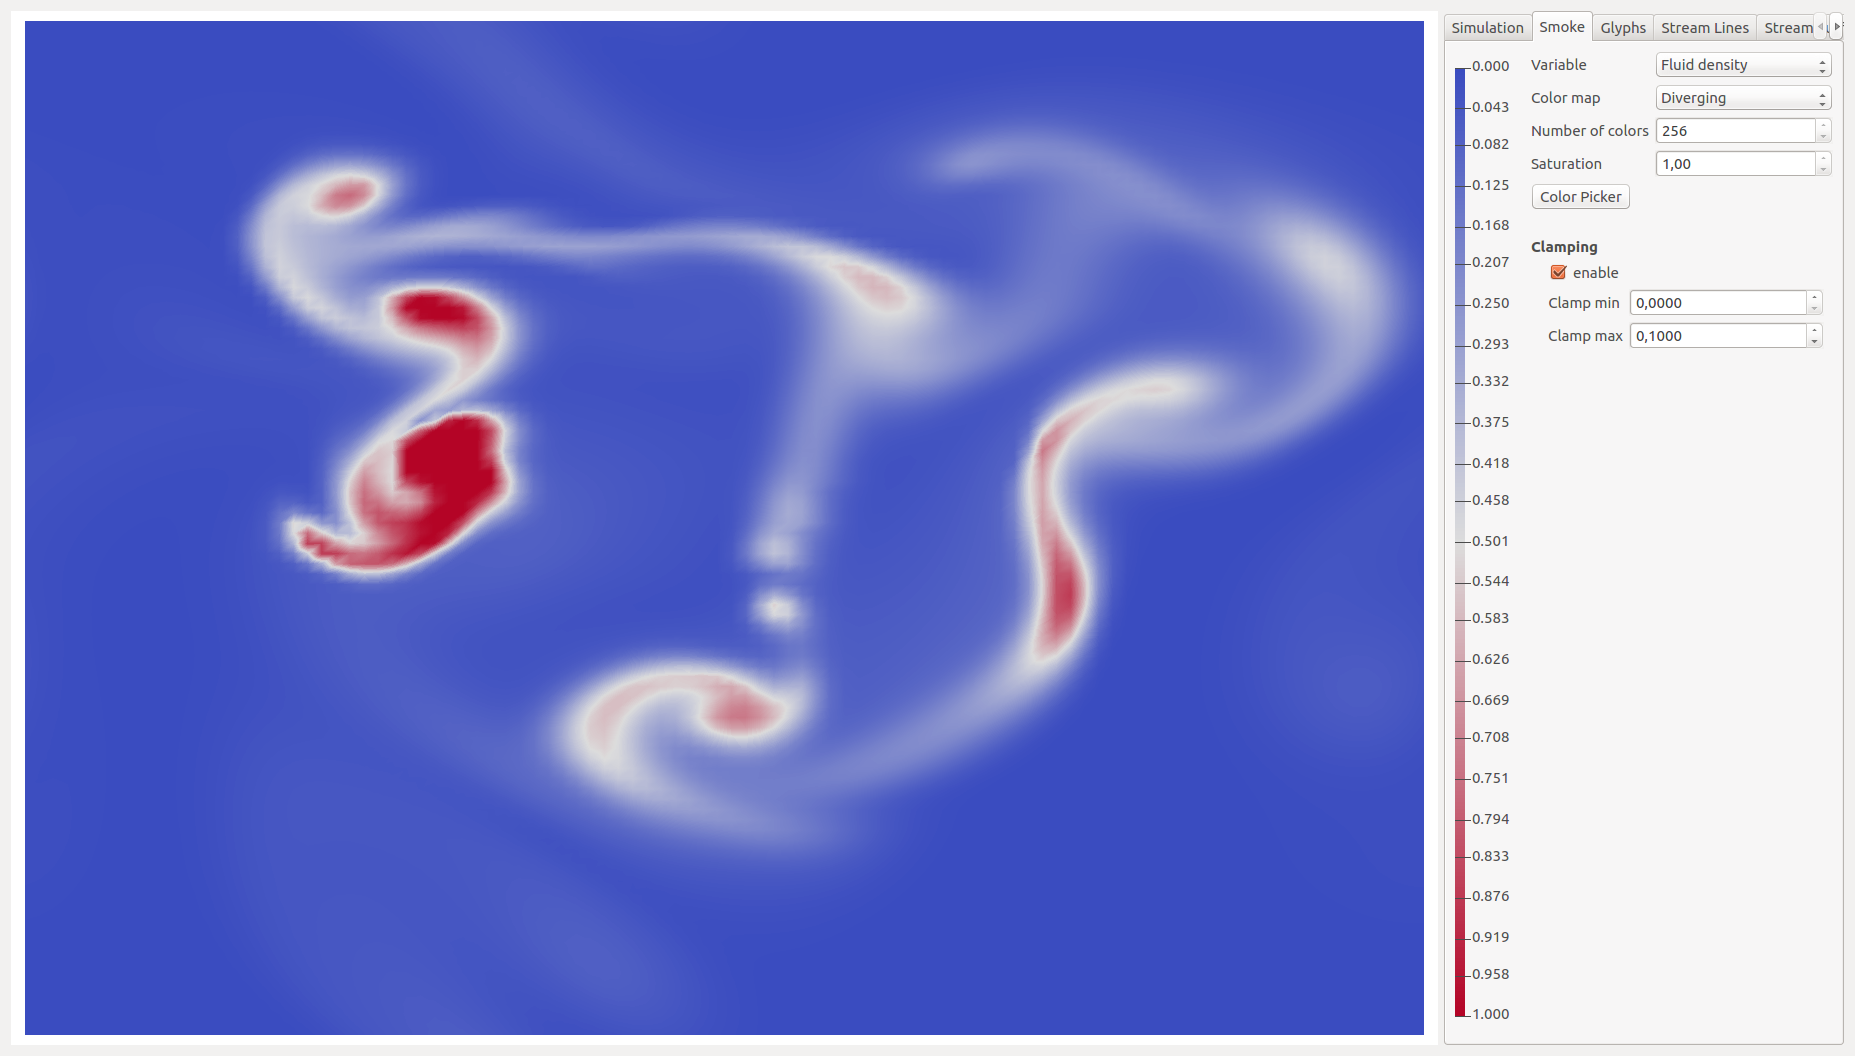
\includegraphics[width=\textwidth, trim={35px 30px 430px 30px}, clip]{colormapping/img/diverging}
		\caption{Blue red diverging colormap.}
		\label{fig:colormapping:intro:differntColorMaps:diverging}
	\end{subfigure}				

	\caption{A visualization of the \emph{Fluid Density} using different colormaps available in the application. All colormaps the full range of available}
	\label{fig:colormapping:colormaps}
\end{figure}

\subsection{Parameterization of Color Maps}
	\todo[inline]{Show image of rainbow colormap with variable dx, discuss}
	\todo[inline]{Show image of colormap with variation in hue, discuss}
	\todo[inline]{Show image of colormap with variation in saturation discuss}

\subsection{Applying Color Maps}
	\todo[inline]{Show image of simulation with clamping/scaling}
	\todo[inline]{Discuss differences}

% \subsection{Variables that the Color Maps are Applied to}
% 	\todo[inline]{Show colormap of fluid density, discuss}
% 	\todo[inline]{Discuss fluid velocity magnitude, discuss}
% 	\todo[inline]{Discuss force field magnitude, discuss}

%!TEX root = ../scivis_lbaakman_bvanloon.tex